\documentclass[letterpaper]{article} % DO NOT CHANGE THIS
\usepackage[submission]{aaai2027}  % DO NOT CHANGE THIS
\usepackage[hyphens]{url}  % DO NOT CHANGE THIS
\usepackage{graphicx} % DO NOT CHANGE THIS
\urlstyle{rm} % DO NOT CHANGE THIS
\def\UrlFont{\rm}  % DO NOT CHANGE THIS
\usepackage{natbib}  % DO NOT CHANGE THIS AND DO NOT ADD ANY OPTIONS TO IT
\usepackage{caption} % DO NOT CHANGE THIS AND DO NOT ADD ANY OPTIONS TO IT
\frenchspacing  % DO NOT CHANGE THIS
\usepackage{booktabs}
\usepackage{amsmath}
\pdfinfo{
/TemplateVersion (2027.1)
}
\setcounter{secnumdepth}{0}

\title{Repair Without Regression? A Budget-Matched Audit of an Agent-Edited Robot Skill}
\author{
    Anonymous Submission
}
\affiliations{
}

\begin{document}

\maketitle

\begin{abstract}
When a coding agent edits a persistent robot controller to fix a failure, aggregate success can hide losses on scenes the controller used to solve. We study this in a controlled case: the scripted Franka pick-and-place controller in Isaac Sim, which replays exactly for a fixed scene order, so every paired transition is caused by an edit. Edits set bounded controller parameters rather than code. Across two frozen repairs, 48 seeded random edits and 7 distinct edits proposed by four AI models, every edit that improved the target lost old successes, and different edits broke the same fragile scenes. Two pre-registered tests show that an 8-scene suite built from earlier edits' losses catches new regressions about twice as often as random old scenes (14 of 20 random and 6 of 7 agent edits, against 36\% and 39\% expected), although 4 agent edits repeated earlier ones. As a zero-loss gate, the suite also rejects almost every useful edit, because no improvement was loss-free. Whether aggregate and zero-loss admission disagree depended more on the old-scene panel than on the rule: compensating gains seen on a development panel built around the failure vanished on a frozen audit of fresh scenes.
\end{abstract}

\section{Introduction}
Coding agents increasingly improve robot behavior by editing executable controllers in response to simulated or real feedback \citep{kuroki2026closedloop,xiao2026enpire,aphale2026selfrepair}. When the edited artifact is a persistent skill, a repair made for one failure is carried into every later scene. The usual acceptance check---did success go up?---can hide a trade: the revised controller may solve new scenes while failing scenes it used to solve. Because the change in old-scene success equals gains minus losses, ``no aggregate decrease'' and ``no lost successes'' differ only when a repair both breaks and fixes old scenes. For a self-improving agent, that acceptance check is the release step of its update layer: it decides which revisions persist, and a regression check is what attributes a lost success to the update that caused it.

Whether that happens for robot skills, and how admission rules respond, has mostly been argued analytically or in software repair \citep{ma2026validation,gao2026looping}. We contribute a small, tightly controlled robot case study: an exactly replaying simulation setup; a development pilot in which aggregate and zero-loss admission disagreed; a frozen audit on 160 fresh scenes, with gate decisions committed before execution, in which they agreed; a post-hoc population of 26 candidates; a pre-registered test on 24 new edits showing that regressions recur on the same scenes, so a suite built from past losses detects new regressions about twice as often as random old scenes at equal cost, though as a strict gate it rejects most useful edits; and a pre-registered test in which repairs proposed by four AI models behave the same way. We do not propose a new verifier, learning algorithm or safety guarantee; regression testing, history-based test prioritization and paired evaluation are established tools. The contribution is controlled evidence about directional gains and losses, about when the choice of admission objective matters, and that a loss history transfers to an evolving robot skill in this case.

\section{Related Work}
Ma and Wu formalize update admission under evaluation budgets, with analytical and synthetic evaluation \citep{ma2026validation}; we study a simulated-robot instance of their question. Kuroki et al.\ refine closed-loop robot code with simulation feedback \citep{kuroki2026closedloop}, and ENPIRE runs an agentic improvement loop on real robots \citep{xiao2026enpire}. Aphale and Singh show that code-as-policy repair must be compared against resampling baselines \citep{aphale2026selfrepair}, so we make no claim about the proposer and hold candidates fixed across gates. In software agents, Gao et al.\ bind evidence to exact code states \citep{gao2026looping}, Xu and Wu test whether passing validation discriminates a fix \citep{xu2026evidence}, and Zhang et al.\ compare verification designs in agent harnesses \citep{zhang2026verification}. We adopt state-bound evidence and parent replay for a persistent robot skill. In machine learning, losing previously correct behavior is studied as catastrophic forgetting \citep{kirkpatrick2017forgetting} and as negative flips between model versions \citep{yan2021pct}. Software regression testing prioritizes tests \citep{elbaum2002prioritization}, including by their history over past releases \citep{kim2002history}; we test that idea with physical scenes and controller edits.

\section{Setup}
\paragraph{Controller and evaluator.} We use Isaac Sim 6.2's scripted Franka pick-and-place controller \citep{nvidia2026franka} with CPU physics at 60\,Hz, one cube, a fixed place goal and an 1{,}800-step horizon. Edits set six bounded high-level parameters, not code: approach height, lift height, motion and grasp convergence tolerances, stability duration and gripper dwell. Motion generation, scenes and the evaluator cannot be edited. Success $S(p,x)\in\{0,1\}$ for controller $p$ on scene $x$ is scored from simulator object state, independently of the controller's completion flag. The cube must be lifted above 7.58\,cm and the episode must end before the horizon; over 30 settling frames the cube must stay within 3.0\,cm of the goal, released and at rest. Four negative controls (no motion, no grasp, holding at the goal, one-step timeout) are all rejected.

\paragraph{Directional outcomes.} For parent $p$, candidate $p'$ and old scenes $x\sim D_o$, let $L=\Pr[S(p,x)=1, S(p',x)=0]$ and $G=\Pr[S(p,x)=0, S(p',x)=1]$. Then $J_o(p')-J_o(p)=G-L$: an aggregate criterion constrains $G-L$, not $L$. If the parent solves every old scene, then $G=0$ and the two notions coincide; they come apart only when gains offset losses. We report the conditional loss $L/J_o(p)$ alongside $G$, $L$ and the target change.

\paragraph{Gates.} Every rule spends 24 rollouts per candidate; a pair is one parent and one candidate rollout on the same scene. \emph{Aggregate} uses 4 target and 8 old pairs and admits if the target net change is positive and the old net change is at least zero, given at least one parent old success. \emph{Preservation} uses the same pairs and also requires zero old losses. \emph{Target-only} uses 12 target pairs and admits if the target improves. \emph{Frozen} never admits. A rejected candidate leaves the parent deployed. No rule certifies safety: zero losses in eight draws is compatible with a substantial loss rate.

\paragraph{Failure discovery and repairs.} Development scenes were searched in documented, adaptive stages: twelve hand-specified scenes (36/36 successes); a radial grid of pick radii 0.35, 0.55 and 0.75\,m at angles from $-60^\circ$ to $60^\circ$ in $30^\circ$ steps (44/45); and a boundary ring at 0.80 and 0.85\,m (0/30). The first scene in manifest order that failed at least two of three resets became the target: radius 0.80\,m, angle $-60^\circ$. The arm stalls in the lift phase with 2.0\,cm residual error against a 1.5\,cm convergence tolerance and times out. A coding assistant inspected the controller source and failure traces and proposed two single-parameter repairs, hashed before execution: \textbf{A} lowers the lift height from 0.30 to 0.20\,m, and \textbf{B} relaxes the motion convergence tolerance from 0.015 to 0.025\,m. The proposals were interactive, so we treat them as fixed artifacts.

\section{Development Pilot}
Each candidate and a fresh parent ran the 25 radial and ring scenes, three resets each, in identical order: 75 labeled rollouts per configuration. Label by label, the parent's discovery run and its repeat agree on all 75 outcomes, with final placement errors within 22\,$\mu$m. Resets within one process differ slightly, but the ordered sequence reproduces exactly across processes, so exact replay holds for a fixed scene order. Paired transitions in a shared order are therefore deterministic consequences of an edit.

Both repairs fixed the target on all three resets. Of the 72 old labels, 44 are parent successes; A lost 4 of them and gained 10 parent failures (net $+6$), and B lost 1 and gained 13 (net $+12$). Applied to the full panel as a diagnostic, aggregate admission accepts both and preservation rejects both. Most gains, however, come from the target's own failure family: 9 of A's and 12 of B's are other 0.80\,m scenes with the same lift stall. Every loss is a placement regression, with the cube at rest 3.4--4.0\,cm from the goal. Re-scoring shows the losses persist at tolerances of 2.0--3.5\,cm and vanish at 4.0\,cm.

\section{Frozen Audit}
\paragraph{Design.} Before any audit rollout, we froze and hashed the protocol, scene manifests and gate and analysis scripts. Target scenes are drawn around the development target: radius in $[0.79, 0.81]$\,m and angle in $[-62^\circ, -58^\circ]$. Old scenes are drawn uniformly over the development region, radius in $[0.35, 0.85]$\,m and angle in $[-60^\circ, 60^\circ]$, excluding a box around the target. A validation draw of 12 target and 8 old scenes was run first, and the gate decisions it produced were written to disk 22\,s before the first audit rollout. The audit itself has 40 target and 120 old scenes, one reset each, in one shuffled order shared by all configurations.

Useful updates were declared in advance: target net change positive and old net change at least zero (aggregate objective), plus zero audit losses (preservation); a secondary objective tolerates a 5\% conditional loss. Repeating the validation parent at the end of the queue reproduced all 20 outcomes, with identical errors. One infrastructure amendment, a launcher fix made before any rollout, left the protocol unchanged.

\begin{figure}[t]
\centering
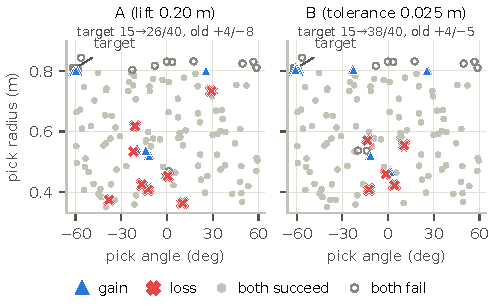
\includegraphics[width=\columnwidth]{fig_audit_map}
\caption{Paired audit outcomes by pick angle and radius. Each marker is one scene. Losses (red) lie in the workspace interior, far from the repaired boundary target (box at upper left). Most scenes that both controllers fail lie beyond 0.80\,m.}
\label{fig:map}
\end{figure}

\begin{table}[t]
\centering
\small
\setlength{\tabcolsep}{1.9pt}
\begin{tabular}{lcccccc}
\toprule
 & Target & Old & \multicolumn{2}{c}{Old} & Cond.\ loss, \% & Useful \\
\cmidrule(lr){4-5}
 & /40 & /120 & gain & loss & [95\% CI] & agg./pres. \\
\midrule
Parent & 15 & 106 & -- & -- & -- & -- \\
A: lift 0.20\,m & 26 & 102 & 4 & 8 & 7.5 [3.9, 14.2] & no/no \\
B: tol.\ 0.025\,m & 38 & 105 & 4 & 5 & 4.7 [2.0, 10.6] & no/no \\
\bottomrule
\end{tabular}
\caption{Frozen audit: 40 target and 120 old scenes, one reset each, paired against the parent. Conditional loss is losses divided by parent old successes, with a Wilson interval over scenes for this single context. Usefulness follows the objectives declared before the audit.}
\label{tab:audit}
\end{table}


\paragraph{Target neighborhood.} Table~\ref{tab:audit} gives the audit outcomes. The parent already succeeds on 15/40 target-neighborhood scenes, all at radius below 0.80\,m. Its 25 failures split into 11 lift stalls and 14 approach timeouts, a mode the development target never showed. A repairs every lift stall but no approach timeout, reaching 26/40. B's tolerance applies to all motion phases; it repairs all 11 lift stalls and 12 of the 14 approach timeouts, reaching 38/40. How far a repair generalizes depends on its mechanism, which three development resets of one scene could not reveal.

\paragraph{Old scenes.} The parent solves 106/120 old scenes; 9 of its 14 failures are approach timeouts beyond 0.80\,m, of which B fixes one and A none. A loses 8 old successes and gains 4, for a net change of $-4$; B loses 5 and gains 4, for a net change of $-1$. The losses lie in the interior, at radii from 0.36 to 0.73\,m (Figure~\ref{fig:map}). All are placement regressions: the parent's errors of 1.3--3.0\,cm become 3.0--4.7\,cm. Unlike in development, they do not vanish at a 4\,cm tolerance, where 2 and 3 losses remain. Neither is useful under the aggregate or zero-loss objective; B is useful under the 5\% tolerance.

\paragraph{Gates.} In the committed validation draw, each candidate lost one of eight old scenes and gained none. Aggregate and preservation therefore both rejected both candidates and kept the parent. Target-only admitted both and delivered B, trading 23 target gains for 5 old losses and 4 old gains. Over 5{,}000 resampled validation draws, aggregate and preservation disagree in only 6.4\% (A) and 5.8\% (B), while target-only admits in at least 99\%.

\paragraph{Why the compensation disappeared.} The development panel was dominated by the boundary ring: 9 of its 24 old scenes lay at 0.80\,m or beyond, four sharing the target's lift stall, against 10 of 120 under uniform sampling. A panel built around the repaired failure over-represents its family and inflates compensating gains, exactly when aggregate admission tolerates losses.

\section{Post-hoc Extension: A Candidate Population}
\paragraph{Design.} After the audit results were known, we froze and hashed a second protocol to ask whether its patterns hold beyond two candidates. It adds 24 edits drawn with a fixed seed from the same interface, each changing one or two parameters to values drawn uniformly within their bounds. They form a non-agent proposal distribution and say nothing about proposer quality. A and B are re-tested unchanged on fresh validation (12 target, 8 old) and audit (30 target, 90 old) draws from the same populations, using the unchanged gate and analysis scripts. Gate decisions were committed before the first audit rollout; all 3{,}800 rollouts completed without retries, and the parent repeat reproduced all 20 outcomes.

\begin{table}[t]
\centering
\small
\setlength{\tabcolsep}{3.0pt}
\begin{tabular}{lccccc}
\toprule
 & \multicolumn{3}{c}{Admitted} & \multicolumn{2}{c}{Agg.-useful} \\
\cmidrule(lr){2-4}\cmidrule(lr){5-6}
Gate & no. & w/ loss & losses & adm. & missed \\
\midrule
\multicolumn{6}{l}{\emph{Post-hoc population: 26 candidates, 7 agg.-useful}} \\
Target-only & 10 & 10 & 61 & 7 & 0 \\
Aggregate & 5 & 5 & 33 & 4 & 3 \\
Preservation & 4 & 4 & 17 & 4 & 3 \\
\midrule
\multicolumn{6}{l}{\emph{Pre-registered test: 24 new edits, 10 agg.-useful}} \\
Target-only & 8 & 8 & 31 & 8 & 2 \\
Uniform suite, 8 & 7 & 7 & 28 & 7 & 3 \\
History suite, 4 & 2 & 2 & 6 & 2 & 8 \\
History suite, 8 & 1 & 1 & 2 & 1 & 9 \\
\bottomrule
\end{tabular}
\caption{Committed gate decisions in the two candidate populations, scored on each population's audit (30 target and 90 old scenes; the parent solves 73 old scenes in both). Losses are summed over admitted candidates. No candidate in either population is useful under the zero-loss objective. Suite gates spend 4 target and $k$ old pairs and admit only with a target gain and zero suite losses. In the pre-registered test, target-only uses the same 4 target pairs, not 12.}
\label{tab:gates2}
\end{table}


\paragraph{Every target improvement lost old successes.} Ten of the 26 candidates improve the target neighborhood, and all ten lose some of the parent's 73 old successes (10/10; Wilson 95\% interval 72--100\%). Their 61 losses are all placement regressions at radii below 0.80\,m.

\paragraph{Gates.} Target-only admitted exactly the ten target improvers, with 61 old losses (Table~\ref{tab:gates2}). Aggregate admitted five and preservation four, every one with audit losses (33 and 17). The two rules disagree in committed decisions only on r14, which fixes all 30 target scenes but loses 16 old successes (net $-6$), and in 3\% of resampled validation draws on average. All three gates delivered B.

\paragraph{A and B on a new draw.} Their target gains replicate (from 10/30 to 15/30 and 27/30), and so does the conditional loss: 8.2\% and 5.5\%, against 7.5\% and 4.7\% in the first audit. The sign of the old net change does not: A and B now gain 8 and 7 old scenes against 6 and 4 losses (net $+2$ and $+3$), mostly interior parent failures just outside the 3\,cm tolerance, of which this draw has 8 among 90 and the first audit 4 among 120.

\section{Pre-registered Test: Loss Histories as Regression Suites}
\paragraph{Hypothesis.} In the population, different edits broke the same old scenes: the 10 most-lost scenes, 14\% of parent successes, carried 42\% of the 163 losses. An evolving agent could then check first the old successes past updates broke. A protocol frozen and pushed to a timestamped repository before any new rollout predicts that, among new edits with audit losses, an 8-scene \emph{history suite} (the scenes most often lost by the 26 earlier candidates) detects a loss more often than 8 scenes drawn uniformly from the parent's 73 old successes are expected to, with the 95\% bootstrap interval of the paired difference above zero.

\paragraph{Design.} Twenty-four new seeded edits from the same generator ran on the population's audit panel, reused by design because a loss history is defined over fixed scenes. Each first ran a 20-scene suite batch (4 target, 8 history and 8 uniform scenes); zero-loss gates on each suite were committed 2\,s before the first audit rollout; every edit then ran the 120-scene audit. All 3{,}520 rollouts completed without retries, and the audit parent reproduced the population's parent on all 120 labels with identical errors.

\begin{figure}[t]
\centering
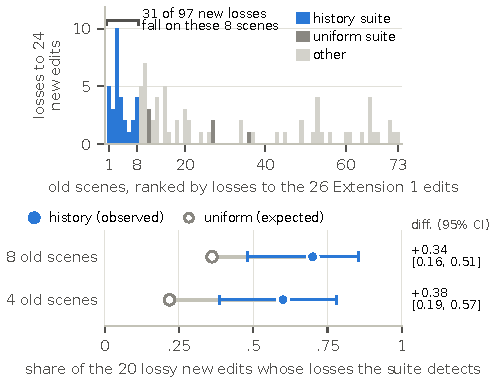
\includegraphics[width=\columnwidth]{fig_ext2}
\caption{Pre-registered test on 24 new edits. Top: losses per old scene, with scenes ranked by how often the 26 earlier candidates lost them; the first eight form the history suite. Bottom: share of the 20 lossy new edits whose losses the suite detected, for the history suite as observed (Wilson 95\% interval) and a uniform suite as expected. Right: paired difference, bootstrap 95\% interval.}
\label{fig:ext2}
\end{figure}


\paragraph{Regressions recur.} Twenty new edits lost old successes, 97 in all, including all 11 that improved the target. Pooled with the population, 21 of 21 target-improving candidates lost old successes (Wilson 85--100\%). The history suite detected a loss in 14 of the 20, against 36\% expected for a uniform suite: a difference of $+0.34$ [0.16, 0.51], so the hypothesis is supported (Figure~\ref{fig:ext2}). With four scenes the rates are 0.60 and 0.22. A third of all new losses (31/97) fell on the eight history scenes. The suite is not merely a fragility proxy (post hoc): the parent's own placement margin ranked lost scenes well on the first audit (AUC 0.81) but at chance in the population the suite was built from (0.49). The one uniform suite we drew detected 7 of 20 (exact McNemar $p=0.09$ against the history suite). Suite batches ran scenes in a different order from the audit, and candidates flipped on 17 of 384 near-threshold labels; reading detection from the audit (post hoc) gives 15 of 20.

\paragraph{Admission.} Used as a zero-loss gate, the history suite is strict (Table~\ref{tab:gates2}). It admitted one edit, with 2 audit losses, where the uniform suite admitted seven with 28. Because no edit improved the target without a loss, it also rejected 9 of the 10 edits useful under the aggregate objective.

\section{Pre-registered Test: Agent-Proposed Repairs}
Under a further protocol frozen and pushed before any agent call, Claude Opus, Sonnet and Haiku~5.5 (Claude Code) and a GPT model (Codex CLI) each received the controller source, bounds and target failure in an empty directory with tools disabled, twice without history and twice with a table of the 50 earlier candidates' gains and losses; a planned fifth agent was unavailable. The 16 answers reduce to 7 distinct edits, run on the same audit panel. All 7 improved the target (by 5--20 of 20 parent failures) and lost 2--6 of the 73 old successes while gaining 6--9; pooled, all 24 distinct target improvers lost old successes. A history suite built likewise from all 50 earlier candidates detected a loss in 6 of 7, against 39\% expected for a uniform suite ($+0.47$ [0.12, 0.68]), as predicted. But the agents stayed near past edits: blind agents rediscovered A and B, and history-prompted agents mostly copied the past edit that fixed the whole target with the fewest losses (2), cutting losses per answer from 4.6 to 2.9 without finding a loss-free repair. Only 3 edits are new (2 detected); rebuilding the suite without each repeat's own history (post hoc) changes nothing.

\section{Discussion and Limitations}
\begin{itemize}
\item Aggregate success hides losses only when gains offset them, and whether they do depends on the old panel: panels inherited from failure discovery can manufacture the offset, and two uniform draws gave opposite net signs for the same repairs while their conditional loss rates agreed. At a 12-pair budget the two rules rarely disagree, and no gate admitted a loss-free improvement because none of the 53 distinct audited edits was one.
\item Regressions are not spread evenly: edits broke the same fragile placements again and again, so the record of past losses was a free regression suite that nearly doubled detection at equal cost. An evolving agent's memory should record what its updates broke, not only what they fixed.
\item Whether B (23 and 17 target gains, 5 and 4 old losses across the two audits) should be deployed has no evidence-only answer; the loss tolerance must be declared first, and a history gate makes that choice sharper, not easier.
\end{itemize}

These observations come from one robot, one task and one repair context. The two repairs were proposed interactively and both populations use random edits. The agent test samples four models twice per prompt, without simulator access, and yields only 3 new edits; both pre-registered tests reuse one scene panel. We make no claim about agent competence, which gate is better in general, or whether loss histories transfer to edits unlike past ones, other skills or a redrawn panel. Parameter edits to a scripted controller are neither code changes nor learned-policy updates, and simulation says nothing about physical safety.

\paragraph{Reproducibility.} An anonymized artifact, released after review, contains the runner, manifests, all rollout records, agent transcripts, frozen hashes, table and figure scripts, and a dependency-free protocol implementation.

\bibliography{refs}

\end{document}
